\documentclass[a4paper,12pt]{scrartcl}
\usepackage[utf8]{inputenc}
\usepackage[UKenglish]{isodate}
\usepackage{csquotes}
\usepackage{graphicx}
\usepackage{wrapfig}
\usepackage{enumitem}
\usepackage{pdflscape}
\usepackage[toc,page]{appendix}
\usepackage{geometry}
\usepackage{hyperref}
\usepackage{cleveref}
\usepackage{listings}
\usepackage{csvsimple}
\usepackage{booktabs}
\usepackage{longtable}
\usepackage{caption}
\usepackage{subcaption}
\usepackage[colorinlistoftodos]{todonotes}
\usepackage[british]{babel}
\usepackage{float}
%\usepackage[margin=1in]{geometry}
\usepackage{listings}
\usepackage{color}
 
\definecolor{codegreen}{rgb}{0,0.6,0}
\definecolor{codegray}{rgb}{0.5,0.5,0.5}
\definecolor{codepurple}{rgb}{0.58,0,0.82}
\definecolor{backcolour}{rgb}{0.95,0.95,0.92}
 
\lstdefinestyle{mystyle}{
	language=PHP,
    backgroundcolor=\color{backcolour},   
    commentstyle=\color{codegray},
    keywordstyle=\color{magenta},
    numberstyle=\tiny\color{codegray},
    stringstyle=\color{codegreen},
    basicstyle=\footnotesize,
    breakatwhitespace=false,         
    breaklines=true,                 
    captionpos=b,                    
    keepspaces=true,                 
    numbers=left,                    
    numbersep=5pt,                  
    showspaces=false,                
    showstringspaces=false,
    showtabs=false,                  
    tabsize=3,
    morekeywords={ new, __halt_compiler, abstract, and, array, as, break, callable, case, catch, class, clone, const, continue, declare, default, die, do, echo, else, elseif, empty, enddeclare, endfor, endforeach, endif, endswitch, endwhile, eval, exit, extends, final, for, foreach, function, global, goto, if, implements, include, include_once, instanceof, insteadof, interface, isset, list, namespace, new, or, print, private, protected, public, require, require_once, return, static, switch, throw, trait, try, unset, use, var, while, xor}
}

\lstset{language=Java,
  showspaces=false,
  showtabs=false,
  breaklines=true,
  showstringspaces=false,
  breakatwhitespace=true,
  commentstyle=\color{pgreen},
  keywordstyle=\color{pblue},
  stringstyle=\color{pred},
  basicstyle=\ttfamily,
  moredelim=[il][\textcolor{pgrey}]{$$},
  moredelim=[is][\textcolor{pgrey}]{\%\%}{\%\%}
}
 
\lstset{style=mystyle}

\graphicspath{ {images/} }
\usepackage[
	backend=biber,
	style=ieee,
	]{biblatex}

\addbibresource{references.bib}

\title{829H1 Real Time Embedded Systems Exercise 1}
\author{Candidate No: 105936}
\date{\today}

\begin{document}
	
	\begin{titlepage}
		\maketitle
	\end{titlepage}
	
	\tableofcontents
	\newpage
	
	\section{Introduction}
	{
		This report outlines the work completed during the laboratory sessions, what equipment was used and what was learnt. Code listings for some of the created programs can be found in \cref{Appendix:start}.
	}

	\section{Equipment}
	{
		\subsection{Hardware}{
			The experiments carried out in this report were run on the Freedom-K64F prototyping board\cite{nxpproducts2014}. To use this board we needed to connect the board to the computer using the debug port and copy across the program we wish to run and then press the reset button to load the program.
			\begin{figure}[h]
				\centering
				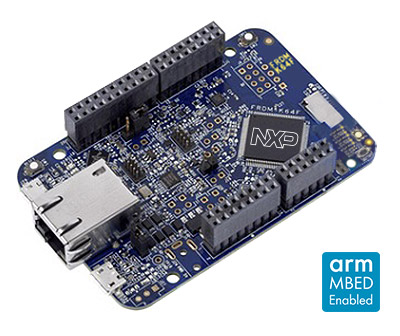
\includegraphics[width=0.5\textwidth]{FRDM-K64F-ANGLE}
				\caption{An Image of the Freedom-K64F Board used during experimentation\cite{nxpproducts2014}}
				\label{img:FRDM-K64F}
			\end{figure}
			Also in the last experiment we used and Oscilloscope to measure the voltage signals from the board to ensure that the program was working properly.
		}
		\subsection{Software}
		{
			To develop the experiments I used Arm's mbed cloud IDE. This allows users to write c++ code and compile it to a device of their choice. 
		}
	}
	
	\section{Experiments}
	{
		\subsection{Digital Output}
		{
			This section will look into programming the digital outputs of the Freedom-K64F board. More specifically I set the LED on the board to turn on and off every second.
			\subsubsection{Adding Comments}
			{
				After adding some comments to the program to describe the code better there was no observable change in the program behaviour. 
			}
			\subsubsection{Varying the Wait Parameter}
			{
				Changing the wait parameter appeared to change the time between the LED turning on and off on the board.
			}
			\subsubsection{Varying the Wait Function}
			{
				In addition to initially using the \lstinline|wait()| function I also used the \lstinline|wait_ms()| which allowed me to specify the wait time in milliseconds. The code for this part can be found in \cref{appendix:ex1-1}
			}
			\subsubsection{Using Different LEDs}
			{
				I also attempted to use different LEDs rather than just LED2 I discovered that LED1 is red, LED2 is green and LED3 is blue. LED4 is also red for some reason although I was expecting it to be white.
			}
			\subsubsection{Using Multiple LEDs Together}
			{
				This worked surprisingly nicely as the LEDs were close enough that setting colours to be on at the same time meant that they would combine for example I was able to combine red and green to make yellow. I was also able to combine all of them to make white. A couple of programs demonstrating this can be found in \cref{appendix:ex1-2} and \cref{appendix:ex1-3}.
			}
			\subsubsection{Why set the value of the LEDs to 1 and 0}
			{
				This is because the LEDs appear to be connected in a open drain mode which means that if I provide a current to the led it turns off.
			}
		}
		\subsection{While Loop}
		{
			The while loop allows for the code inside the loop to be continuously run while the statement for the loop is true.
			\subsubsection{Using ++ and -- operators}
			{
				This is a shorthand way of writing \lstinline|i = i + 1| and \lstinline|i = i - 1| this makes sense as incrementing and decrementing are very easy for computers to do which means that having a shorthand way of writing it means it can be translated in to the computer code more efficiently. It is also possible to use \lstinline|+=| and \lstinline|-=| which allow you to add and subtract values from variables.
			}
			\subsubsection{Replacing myled=1 with myled.write(1)}
			{
				This has the same function I believe what is happening is that the \lstinline|DigitalOut| class overloads the assignment operator so that \lstinline|.write()| is called on the value is assigned to the object. The program for this experiment can be found in \cref{appendix:ex2-1}.
			}
		}
		\subsection{Digital Input}
		{
			This consisted of using everything I had learnt so far and also using the value of the \lstinline|SW2| switch to change the function of the lights. This was quite simple as all you have to do is call the read function on the input you wish and the value is provided. A program which changed the colour of the light if you press the switch can be found at \cref{appendix:ex3-1}. The slightly difficult task was creating the oscilloscope program as I had to find out the time period needed for a 100hz and 200hz frequency and then all I had to do was set the value of the pin. I used the PTC16 port on the board to output the current to, this was identified using \cref{img:FRDM-K64F-HEADERPINS}. This program can be found at \cref{appendix:ex3-2}
			\begin{figure}
				\centering
				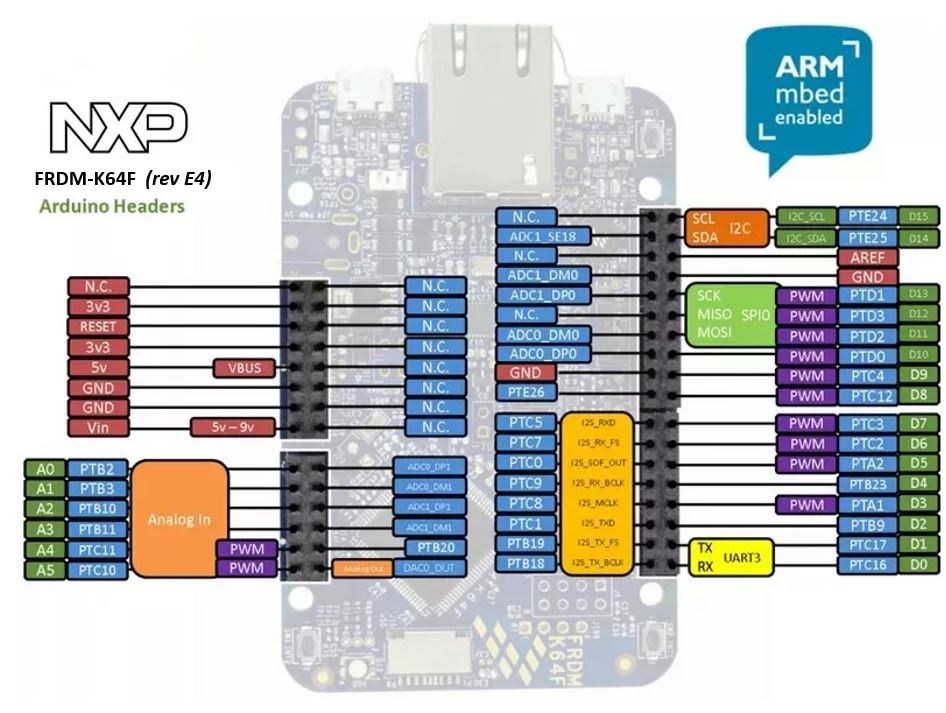
\includegraphics[width=\textwidth]{frdm_k64f_reve4_header_pinout}
				\caption{An Image of the Freedom-K64F Board with the codes for the header pins overlaid\cite{armlimited2015}}
				\label{img:FRDM-K64F-HEADERPINS}
			\end{figure}
		}
	}

	\section{Conclusion}
	{
		In conclusion a lot was learnt and the ability to interface with the different components on the board has grown. Also knowledge about how to develop on embedded systems has been attained and should provide a useful starting ground for future development.
	}
	
	\newpage
	\begin{appendices}
	\label{Appendix:start}
	\section{Lab Exercise 1}
	{
		\subsection{Part 1}
		{
			\label{appendix:ex1-1}
			\lstinputlisting[language=c++]{CodeListings/Ex1/mainPart1.cpp}
		}
		\subsection{Part 2}
		{
			\label{appendix:ex1-2}
			\lstinputlisting[language=c++]{CodeListings/Ex1/mainPart2.cpp}
		}
		\subsection{Part 3}
		{
			\label{appendix:ex1-3}
			\lstinputlisting[language=c++]{CodeListings/Ex1/mainPart3.cpp}
		}
	}
	\section{Lab Exercise 2}
	{
		\label{appendix:ex2}
		\subsection{Part 1 - Master Program}
		{
			\label{appendix:ex2-1}
			\lstinputlisting[language=c++]{CodeListings/Ex2/main-master.cpp}
		}
		\subsection{Part 2 - Slave Program}
		{
			\label{appendix:ex2-2}
			\lstinputlisting[language=c++]{CodeListings/Ex2/main-slave.cpp}
		}
	}

\end{appendices}
	\printbibliography[heading=bibintoc,title=References]
\end{document}
